\documentclass[12pt, titlepage]{article}

% Author's up-front packages
\usepackage[T1]{fontenc}
\usepackage[utf8]{inputenc}
\usepackage{longtable}

%Packages on template
\usepackage{fullpage}
\usepackage{multirow}
\usepackage{booktabs}
\usepackage{tabularx}
\usepackage{graphicx}
\usepackage{float}
% Personal addtion
\usepackage{xr-hyper}
% End Personal addtion
\usepackage{hyperref}

% Author's packages

\usepackage{amsmath, mathtools}
\usepackage{amsfonts}
\usepackage{amssymb}
\usepackage{graphicx}
\usepackage{cite}
\usepackage{indentfirst}
\usepackage{float}
\usepackage{csquotes}
\usepackage{cleveref}

%Hypersetup on template
\hypersetup{
    colorlinks,
    citecolor=black,
    filecolor=black,
    linkcolor=red,
    urlcolor=blue
}

\newcommand{\progname}{STEM Moir{\'e} GPA}
\externaldocument[SRS:]{../../SRS/SRS}
\externaldocument[TP:]{../../TestPlan/TestPlan}

% Author choice to remove
% \usepackage[round]{natbib}

%% Comments

\usepackage{color}

\newif\ifcomments\commentstrue

\ifcomments
\newcommand{\authornote}[3]{\textcolor{#1}{[#3 ---#2]}}
\newcommand{\todo}[1]{\textcolor{red}{[TODO: #1]}}
\else
\newcommand{\authornote}[3]{}
\newcommand{\todo}[1]{}
\fi

\newcommand{\wss}[1]{\authornote{blue}{SS}{#1}}
\newcommand{\an}[1]{\authornote{magenta}{Author}{#1}}


\newcommand{\mref}[1]{M\ref{#1}}


%Set the custom referencing system (author's initiative)
	% Anticipated Changes
\newtheorem{AC}{AC}
\crefname{AC}{AC}{ACs}
	% Unlikely Changes
\newtheorem{UC}{UC}
\crefname{UC}{UC}{UCs}
	% Module
\newtheorem{M}{M}
\crefname{M}{M}{Ms}
	% Requirement
\newtheorem{R}{R}
\crefname{R}{R}{Rs}

\begin{document}

\title{Module Guide (MG) \\
STEM Moir{\'e} GPA} 
\author{Alexandre Pofelski \\
		macid: pofelska \\
		github: slimpotatoes}
\date{\today}

\maketitle

\pagenumbering{roman}

\section{Revision History}

\begin{table}[h]
\caption{\bf Revision History}
\begin{tabularx}{\textwidth}{p{3cm}p{2cm}X}
\toprule {\bf Date} & {\bf Version} & {\bf Notes}\\
\midrule
5/11/2017 & 1.0 & First Draft\\
14/11/2017 & 1.1 & Object Structure Module removed \\
26/11/2017 & 1.2 & \cref{AC_Assum_SmallStrain} statement modified to target exclusively \cref{M_StrainCalc} module\\
27/11/2017 & 1.3 & Matched MG to MIS \\
\bottomrule
\end{tabularx}
\end{table}

\newpage
\section{Symbols, Abbreviations and Acronyms}
\label{symbols}

Symbols, Abbreviations and Acronyms used in the Module guide document are regrouped under the following table, in \cref{SRS:table_symbols_SRS} and in \cref{SRS:table_acro_SRS} of the SRS document, and in \cref{TP:table_acro_Test_Plan} of the Test Plan document. Documents are available on \href{https://github.com/slimpotatoes/STEM_Moire_GPA}{\progname{}} repository. \par\bigskip

\renewcommand{\arraystretch}{1.2}
\begin{tabular}{l l} 
  \toprule		
  \textbf{symbol} & \textbf{description}\\
  \midrule 
  GPA & Geometrical Phase Analysis \\
  LSFM & Least Square Fit Method \\
  FT & Fourier Transform \\
  \bottomrule
  \label{table_acro_Test_Plan}
\end{tabular}

\newpage

\tableofcontents

\listoftables

\listoffigures

\newpage

\pagenumbering{arabic}

\section{Introduction}

%Keep as comment
\iffalse
Decomposing a system into modules is a commonly accepted approach to developing
software.  A module is a work assignment for a programmer or programming
team~\cite{ParnasEtAl1984}.  We advocate a decomposition
based on the principle of information hiding~\cite{Parnas1972a}.  This
principle supports design for change, because the ``secrets'' that each module
hides represent likely future changes.  Design for change is valuable in SC,
where modifications are frequent, especially during initial development as the
solution space is explored.  

Our design follows the rules layed out by \cite{ParnasEtAl1984}, as follows:
\begin{itemize}
\item System details that are likely to change independently should be the
  secrets of separate modules.
\item Each data structure is used in only one module.
\item Any other program that requires information stored in a module's data
  structures must obtain it by calling access programs belonging to that module.
\end{itemize}

After completing the first stage of the design, the Software Requirements
Specification (SRS), the Module Guide (MG) is developed~\cite{ParnasEtAl1984}. 
The MGspecifies the modular structure of the system and is intended to allow 
bothdesigners and maintainers to easily identify the parts of the software. The
potential readers of this document are as follows:

\begin{itemize}
\item New project members: This document can be a guide for a new project member
  to easily understand the overall structure and quickly find the
  relevant modules they are searching for.
\item Maintainers: The hierarchical structure of the module guide improves the
  maintainers' understanding when they need to make changes to the system. It is
  important for a maintainer to update the relevant sections of the document
  after changes have been made.
\item Designers: Once the module guide has been written, it can be used to
  check for consistency, feasibility and flexibility. Designers can verify the
  system in various ways, such as consistency among modules, feasibility of the
  decomposition, and flexibility of the design.
\end{itemize}
\fi
%End comment

The module guide document is providing to the reader the decomposition of 
\progname{} into smaller pieces to help the implementation phase. The 
decomposition is based on the principle of information hiding~\cite{Parnas1972a} 
which interest relies on its flexibility to design change. The module design 
follows the rules layed out by \cite{ParnasEtAl1984}, as follows:
\begin{itemize}
\item System details that are likely to change independently should be the
  secrets of separate modules.
\item Each data structure is used in only one module.
\item Any other program that requires information stored in a module's data
  structures must obtain it by calling access programs belonging to that module.
\end{itemize}

The module guide (MG) follows the Software Requirements Specification (SRS) 
available in the documentation tree. Terminologies, symbols and acronyms used in 
the document are described in the SRS and TestPlan documents. The rest of the 
document is organized as follows. \Cref{SecChange} lists the anticipated and 
unlikely changes of the software requirements. \Cref{SecMH} summarizes the 
module decomposition that was constructed according to the likely changes. 
\Cref{SecConnection} specifies the connections between the software requirements 
and the modules. \Cref{SecMD} gives a detailed description of the modules. 
Section \cref{SecTM} includes two traceability matrices. One checks the 
completeness of the design against the requirements provided in the SRS. The 
other shows the relation between anticipated changes and the modules. 
\Cref{SecUse} describes the use relation between modules.

\section{Anticipated and Unlikely Changes} \label{SecChange}

This section lists possible changes to the system. According to the likeliness
of the change, the possible changes are classified into two
categories. Anticipated changes are listed in \cref{SecAchange}, and
unlikely changes are listed in \cref{SecUchange}.

\subsection{Anticipated Changes} \label{SecAchange}

Anticipated changes are the source of the information that is to be hidden
inside the modules. Ideally, changing one of the anticipated changes will only
require changing the one module that hides the associated decision. 

\begin{AC}\normalfont Hardware on which is \progname{} running
\label{AC_Hardware}
\end{AC}

\begin{AC}\normalfont 
$I_{\mathit{SMH}_{\texttt{exp}}},I_{\mathit{C}_{\texttt{ref}}}$ inputs file 
format
\label{AC_FormatFile}
\end{AC}

\begin{AC}\normalfont Gradient of displacement field tensor decomposition
  \wss{You think you will likely change this assumption?  I see that it is
    linked to a 2D strain tensor module.  Can you really isolate this change to
    one module?  I am not familiar enough with your area, but I have prior
    experience with continuum mechanics and computational mechanics.  The switch
    from a small strain tensor to one of the several available finite
    deformation tensors would have a greater impact than just changing the
    values in one tensor.}
    \an{I agree. AC statement changed to target the module}
\label{AC_Assum_SmallStrain}
\end{AC}

\begin{AC}\normalfont SMH simulation from a reference algorithm
\label{AC_SMH_algo}
\end{AC}

\begin{AC}\normalfont GPA algorithm
\label{AC_GPA_algo}
\end{AC}

\begin{AC}\normalfont Mask function for frequency isolation (in GPA)
\label{AC_Mask}
\end{AC}

\begin{AC}\normalfont Fitting algorithm to get unstrained reference 
\label{AC_RefFit}
\end{AC}

\begin{AC}\normalfont Output format
\label{AC_Output}
\end{AC}

\begin{AC}\normalfont Internal Data strucutre
\label{AC_Data}
\end{AC}

\iffalse
\begin{AC}\normalfont Internal Object strucutre
\label{AC_Object}
\end{AC}
\fi

\subsection{Unlikely Changes} \label{SecUchange}

\iffalse
The module design should be as general as possible. However, a general system is
more complex. Sometimes this complexity is not necessary. Fixing some design
decisions at the system architecture stage can simplify the software design. If
these decision should later need to be changed, then many parts of the design
will potentially need to be modified. Hence, it is not intended that these
decisions will be changed.
\fi

The unlikely changes are design decisions fixing some aspects of \progname{}. 
The lack of modularity is compensated by a simplification in the software 
design. If any of the elements are modified, important changes would be expected 
in the design. Therefore the following decisions are expected to stay unchanged.

\begin{UC}\normalfont SMH data type (2D arrays)
\label{UC_Input_data}
\end{UC}

\begin{UC}\normalfont Perfect 2D periodic scanning grid assumption
\label{UC_Assum_2DPeriodicGrid}
\end{UC}

\begin{UC}\normalfont Pixel data type (real number)
\label{UC_Assum_Pixel}
\end{UC}

\begin{UC}\normalfont Keyboard/mouse interface device with user
\label{UC_Assum_Hardware}
\end{UC}

\section{Module Hierarchy} \label{SecMH}

This section provides an overview of the module design. Modules are summarized
in a hierarchy decomposed by secrets in \cref{TblMH}. The modules listed
below, which are leaves in the hierarchy tree, are the modules that will
actually be implemented.

\begin{M}\normalfont Hardware-Hiding Module (described in \cref{MG_Hardware})
\label{M_Hardware}
\end{M}

\begin{M}\normalfont \progname{}  Control Module (described in \cref{MG_Control})
\label{M_Control}
\end{M}

\begin{M}\normalfont \progname{} GUI Module (described in \cref{MG_GUISMG})
\label{M_GUISMG}
\end{M}

\begin{M}\normalfont User input Module (described in \cref{MG_InputFormat})
\label{M_InputFormat}
\end{M}

\begin{M}\normalfont SMH simulation Module (described in \cref{MG_SMHSim})
\label{M_SMHSim}
\end{M}

\begin{M}\normalfont GPA Module (described in \cref{MG_GPA})
\label{M_GPA}
\end{M}

\begin{M}\normalfont Mask Module (described in \cref{MG_Mask})
\label{M_Mask}
\end{M}

\begin{M}\normalfont Unstrained region Module (described in \cref{MG_URef})
\label{M_URef}
\end{M}

\begin{M}\normalfont Conversion Module (described in \cref{MG_MtoCConv})
\label{M_MtoCConv}
\end{M}

\begin{M}\normalfont 2D strain tensor Module (described in \cref{MG_StrainCalc})
\label{M_StrainCalc}
\end{M}

\begin{M}\normalfont Fourier Transform Module (described in \cref{MG_FT})
\label{M_FT}
\end{M}

\begin{M}\normalfont Gradient Module (described in \cref{MG_Gradient})
\label{M_Gradient}
\end{M}

\begin{M}\normalfont Least Square Fitting Method Module (described in \cref{MG_LSFM})
\label{M_LSFM}
\end{M}

\begin{M}\normalfont Phase operation Module (described in \cref{MG_Phase})
\label{M_Phase}
\end{M}

\begin{M}\normalfont Data Structure Module (described in \cref{MG_DataStruct})
\label{M_DataStruct}
\end{M}

\iffalse
\begin{M}\normalfont Object Structure Module (described in \cref{MG_ObjectStruct})
\label{M_ObjectStruct}
\end{M}
\fi

\begin{M}\normalfont Generic GUI/Plot Module (described in \cref{MG_GUIGene})
\label{M_GUIGene}
\end{M}

\begin{table}[H]
\centering
\begin{tabular}{p{0.3\textwidth} p{0.6\textwidth}}
\toprule
\textbf{Level 1} & \textbf{Level 2}\\
\midrule

{Hardware-Hiding Module} & ~ \\
\midrule

\multirow{10}{0.3\textwidth}{Behaviour-Hiding Module} & Input\\
& \progname{} Control \\
& \progname{} GUI \\
& User Input \\
& SMH simulation \\
& GPA \\
& Mask \\
& Unstrained region \\
& Conversion \\
& 2D strain tensor \\
\midrule

\multirow{7}{0.3\textwidth}{Software Decision Module} & Fourier Transform \\
& Least square fitting method \\
& Phase calculation \\
& Gradient \\
& Generic GUI/Plot \\
& Data structure \\
\bottomrule

\end{tabular}
\caption{Module Hierarchy}
\label{TblMH}
\end{table}

\section{Connection Between Requirements and Design} \label{SecConnection}

The design of the system is intended to satisfy the requirements developed in
the SRS. In this stage, the system is decomposed into modules. The connection
between requirements and modules is listed in Table \ref{TblRT}.

\section{Module Decomposition} \label{SecMD}

Modules are decomposed according to the principle of ``information hiding''
proposed by \cite{ParnasEtAl1984}. The \emph{Secrets} field in a module
decomposition is a brief statement of the design decision hidden by the
module. The \emph{Services} field specifies \emph{what} the module will do
without documenting \emph{how} to do it. For each module, a suggestion for the
implementing software is given under the \emph{Implemented By} title. If the
entry is \emph{OS}, this means that the module is provided by the operating
system or by standard programming language libraries.  Also indicate if the
module will be implemented specifically for the software.

Only the leaf modules in the
hierarchy have to be implemented. If a dash (\emph{--}) is shown, this means
that the module is not a leaf and will not have to be implemented. Whether or
not this module is implemented depends on the programming language
selected.

\subsection{Hardware Hiding Modules (\texorpdfstring{\cref{M_Hardware}}))}
\label{MG_Hardware}
\begin{description}
\item[Secrets:]The data structure and algorithm used to implement the virtual 
hardware.
\item[Services:]Serves as a virtual hardware used by the rest of the system. 
This module provides the interface between the hardware and the software. So, 
the system can use it to display outputs or to accept inputs.
\item[Implemented By:] OS
\end{description}


\subsection{Behaviour-Hiding Module}

\iffalse
\begin{description}
\item[Secrets:]The contents of the required behaviours.
\item[Services:]Includes programs that provide externally visible behaviour of
  the system as specified in the software requirements specification (SRS)
  documents. This module serves as a communication layer between the
  hardware-hiding module and the software decision module. The programs in this
  module will need to change if there are changes in the SRS.
\item[Implemented By:] --
\end{description}
\fi

\subsubsection{\progname{} Control Module (\texorpdfstring{\cref{M_Control}}))}
\label{MG_Control}
\begin{description}
\item[Secrets:] Execution flow of \progname{}.
\item[Services:] Calls the different modules in the appropriate order.
\item[Implemented By:] \progname{}
\end{description}

\subsubsection{\progname{} GUI (\texorpdfstring{\cref{M_GUISMG}}))}
\label{MG_GUISMG}
\begin{description}
\item[Secrets:] Methods to interact with user to make run \progname{}.
\item[Services:] Serves as interface between the user and the software through 
the hardware by outputting calculation results and collecting user information 
(user inputs) for the calculation modules. 
\item[Implemented By:] \progname{}
\end{description}

\subsubsection{Input Module (\texorpdfstring{\cref{M_InputFormat}}))}
\label{MG_InputFormat}
\begin{description}
\item[Secrets:] The format and structure of the input data.
\item[Services:] Loads, verifies and stores the input data into the appropriate 
data and object structure.
\item[Implemented By:] \progname{}
\end{description}

\subsubsection{SMH simulation Module (\texorpdfstring{\cref{M_SMHSim}}))}
\label{MG_SMHSim}
\begin{description}
\item[Secrets:] Algorithm to simulate the SMH from the reference image 
$I_{C_{\texttt{Ref}}}$.
\item[Services:] Simulates the SMH in Fourier space using the pixel size $p$ of 
$I_{\mathit{SMH}_{\texttt{exp}}}$ and the Fourier transform the image reference 
$I_{C_{\texttt{ref}}}$.
\item[Implemented By:] \progname{}
\end{description}

\subsubsection{GPA Module (\texorpdfstring{\cref{M_GPA}}))}
\label{MG_GPA}
\begin{description}
\item[Secrets:] GPA algorithm.
\item[Services:] Calculates the variation of masked Moir{\'e} wave vector on 
each element of the array.
\item[Implemented By:] \progname{}
\end{description}

\subsubsection{Mask Module (\texorpdfstring{\cref{M_Mask}}))}
\label{MG_Mask}
\begin{description}
\item[Secrets:] Algorithm to isolate a portion of an image.
\item[Services:] Isolates and weights a sub area of an image by fixing the 
parameter $M_j$.
\item[Implemented By:] \progname{}
\end{description}

\subsubsection{Unstrained region Module (\texorpdfstring{\cref{M_URef}}))}
\label{MG_URef}
\begin{description}
\item[Secrets:] Algorithm to calculate the unstrained reference.
\item[Services:] Calculates the unstrained reference based on the user input $U$ 
and the result of the fitting method.
\item[Implemented By:] \progname{}
\end{description}

\subsubsection{Conversion Module (\texorpdfstring{\cref{M_MtoCConv}}))}
\label{MG_MtoCConv}
\begin{description}
\item[Secrets:] Algorithm to convert a Moir{\'e} wave vector to a crystalline 
wave vector.
\item[Services:] Performs the affine vectorial transformation using the 
Moir{\'e} wave vectors and the sampling vectors as inputs.
\item[Implemented By:] \progname{}
\end{description}

\subsubsection{2D strain tensor Module (\texorpdfstring{\cref{M_StrainCalc}}))}
\label{MG_StrainCalc}
\begin{description}
\item[Secrets:] Algorithm to calculate the strain from distortion matrix.
\item[Services:] Calculates the strain tensor on each pixel of the array.
\item[Implemented By:] \progname{}
\end{description}

\subsection{Software Decision Module}

\subsubsection{Fourier Transform Module (\texorpdfstring{\cref{M_FT}}))}
\label{MG_FT}
\begin{description}
\item[Secrets:] Fourier transform algorithm.
\item[Services:] Transforms data into its Fourier transform.
\item[Implemented By:]Python library
\end{description}

\subsubsection{Gradient Module (\texorpdfstring{\cref{M_Gradient}}))}
\label{MG_Gradient}
\begin{description}
\item[Secrets:] 2D Gradient algorithm.
\item[Services:] Performs the 2D derivative of function.
\item[Implemented By:]Python library
\end{description}

\subsubsection{Least Square Fitting Method Module (\texorpdfstring{\cref{M_LSFM}}))}
\label{MG_LSFM}
\begin{description}
\item[Secrets:] Least Square Fitting algorithm.
\item[Services:] Fits a set of data into a 2D linear function using the Least 
squares method.
\item[Implemented By:] Python library
\end{description}

\subsubsection{Phase Module (\texorpdfstring{\cref{M_Phase}}))}
\label{MG_Phase}
\begin{description}
\item[Secrets:] Algorithm to wrap/unwrap the phase.
\item[Services:] Wraps/unwraps the phase by adding/removing discontinuities in 
the interval [0,2$\pi$].
\item[Implemented By:]Python library
\end{description}

\subsubsection{Data Structure Module (\texorpdfstring{\cref{M_DataStruct}}))}
\label{MG_DataStruct}
\begin{description}
\item[Secrets:] Data format for an image.
\item[Services:] Provides convenient format to store, read and manipulate all 
elements (pixel) from an image.
\item[Implemented By:] Python library
\end{description}

\iffalse
\subsubsection{Object Structure Module (\texorpdfstring{\cref{M_ObjectStruct}}))}
\label{MG_ObjectStruct}
\begin{description}
\item[Secrets:] Format for the object carried by the control module.
\item[Services:] Provides object format usable by module called by the control 
module.
\item[Implemented By:] Python library
\end{description}
\fi

\subsubsection{Generic GUI/Plot Module (\texorpdfstring{\cref{M_GUIGene}}))}
\label{MG_GUIGene}
\begin{description}
\item[Secrets:] Generic methods to interact with the user.
\item[Services:] Provides the generic interface methods such as buttons, 
windows, plotting, entry fields to interact with a user.
\item[Implemented By:] Python library
\end{description}

\section{Traceability Matrix} \label{SecTM}

This section shows two traceability matrices: between the modules and the
requirements and between the modules and the anticipated changes.

% the table should use mref, the requirements should be named, use something
% like fref
\begin{table}[H]
\centering
\begin{tabular}{p{0.2\textwidth} p{0.6\textwidth}}
\toprule
\textbf{Req.} & \textbf{Modules}\\
\midrule
\cref{SRS:R_1} & \cref{M_GUISMG}, \cref{M_Control}, \cref{M_Hardware} \\
\cref{SRS:R_2} & \cref{M_InputFormat} \\
\cref{SRS:R_3} & \cref{M_SMHSim}, \cref{M_Control} \\
\cref{SRS:R_4} & \cref{M_GUISMG}, \cref{M_Hardware} \\
\cref{SRS:R_5} & \cref{M_GUISMG}, \cref{M_Hardware} \\
\cref{SRS:R_6} & \cref{M_InputFormat} \\
\cref{SRS:R_7} & \cref{M_GPA}, \cref{M_Mask}, \cref{M_Control} \\
\cref{SRS:R_8} & \cref{M_GUISMG}, \cref{M_Hardware} \\
\cref{SRS:R_9} & \cref{M_InputFormat} \\
\cref{SRS:R_10} & \cref{M_URef}, \cref{M_Control} \\
\cref{SRS:R_11} & \cref{M_GUISMG}, \cref{M_Hardware} \\
\cref{SRS:R_12} & \cref{M_MtoCConv}, \cref{M_InputFormat}, \cref{M_Control} \\
\cref{SRS:R_13} & \cref{M_StrainCalc} \\
\cref{SRS:R_14} & \cref{M_GUISMG}, \cref{M_Hardware}\\
\bottomrule
\end{tabular}
\caption{Trace Between Requirements and Modules}
\label{TblRT}
\end{table}

\begin{table}[H]
\centering
\begin{tabular}{p{0.2\textwidth} p{0.6\textwidth}}
\toprule
\textbf{AC} & \textbf{Modules}\\
\midrule
\cref{AC_Hardware} & \cref{M_Hardware}\\
\cref{AC_FormatFile} & \cref{M_InputFormat}\\
\cref{AC_Assum_SmallStrain} & \cref{M_StrainCalc}\\
\cref{AC_SMH_algo} & \cref{M_SMHSim}\\
\cref{AC_GPA_algo} & \cref{M_GPA}\\
\cref{AC_Mask} & \cref{M_Mask}\\
\cref{AC_RefFit} & \cref{M_LSFM}\\
\cref{AC_Output} & \cref{M_GUISMG}\\
\cref{AC_Data} & \cref{M_DataStruct}\\
\bottomrule
\end{tabular}
\caption{Trace Between Anticipated Changes and Modules}
\label{TblACT}
\end{table}

\section{Use Hierarchy Between Modules} \label{SecUse}

In this section, the uses hierarchy between modules is
provided. \cite{Parnas1978} said of two programs A and B that A {\em uses} B if
correct execution of B may be necessary for A to complete the task described in
its specification. That is, A {\em uses} B if there exist situations in which
the correct functioning of A depends upon the availability of a correct
implementation of B.  Figure \ref{FigUH} illustrates the use relation between
the modules. It can be seen that the graph is a directed acyclic graph
(DAG). Each level of the hierarchy offers a testable and usable subset of the
system, and modules in the higher level of the hierarchy are essentially simpler
because they use modules from the lower levels.

\begin{figure}[H]
\centering
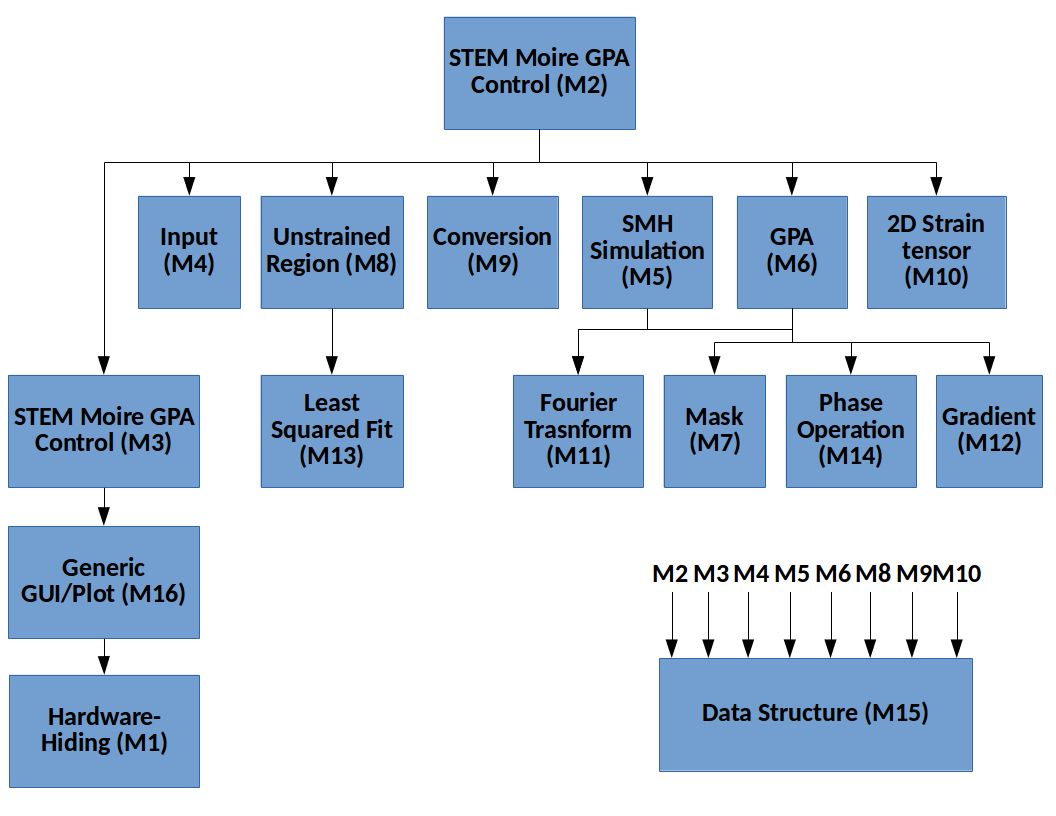
\includegraphics[width=\linewidth]{Figure_Hierarchy_update.png}
\caption{Use hierarchy among modules}
\label{FigUH}
\end{figure}

\newpage

\bibliographystyle{ieeetr}
\bibliography{MG}

\end{document}
